\documentclass[output=paper]{langsci/langscibook} 
\author{Natalia Levshina\affiliation{Leipzig University}}
\title{Linguistic {Frankenstein}, or {How} to test universal constraints without real languages}
\shorttitlerunninghead{Linguistic Frankenstein}
\abstract{The scarcity of diachronic data represents a serious problem when linguists try to explain a typological universal. To overcome this empirical bottleneck, one can simulate the process of language evolution in artificial language learning experiments. After a brief discussion of the main principles and findings of such experiments, this paper presents a case study of causative constructions showing that language users have a bias towards the efficient organisation of communication. They regularise their linguistic input such that more frequent causative situations are expressed by shorter forms, and less frequent situations are expressed by longer forms. This supports the economy-based explanation of the universal form-meaning mapping found in causative constructions of different languages.}
\begin{document}
\maketitle 
 





 
\section{Problems with testing functional explanations}

Functional linguists have formulated many universal principles that are meant to explain the structure and use of human languages, such as the principles of economy, iconicity, cognitive complexity, minimization of domains, avoidance of identity, and so on (e.g. \citealt{Haiman1983}; \citealt{Rohdenburg1996}; \citealt{Rohdenburg2003}; \citealt{Hawkins2004}; \citealt{Haspelmath2008_FreqIcon}). How can one decide which explanation is relevant for a certain cross-linguistic pattern and how does one make sure that the latter is not a result of a historical coincidence in the sense of \citetv{Collins2019tv}? Ideally, we would need data from genealogically and geographically diverse languages over a large time span. Needless to say, this is unrealistic: as a rule, such data are not available. The time depth and typological breadth of available diachronic data are very limited. Moreover, even in an ideal world where any kind of linguistic data is obtainable at the click of a button, this might still be insufficient. First, real language data are observational, which makes a causal interpretation of the correlational results rather difficult (this does not mean there are no successful attempts, e.g. Moscoso del \citealt{Prado2014}). Second, real language is a battleground of various forces, many of which can be mutually exclusive, e.g. over- and underspecification, iconicity and economy-driven arbitrariness, and so on. Disentangling these factors in real ‘messy’ language data is not a trivial task. Moreover, as pointed out by \citet{SmithEtAl2017} in their discussion of the universal bias against free variation, transmission of language in populations can mask the biases of learners: the language in a population might retain variability even though every learner is biased against acquiring such variation. Unless the data contain meta-information about the speakers, these effects may go undetected.

These problems can be solved with the help of the artificial language learning paradigm, which has gained popularity recently. One can observe in real time how linguistic systems undergo change, revealing the cognitive and communicative biases of language users. One can control for some factors while testing those of interest, and study the behaviour of each individual speaker within a population. Similar to the protagonist of Mary Shelley’s gothic novel, Victor Frankenstein, who created a sentient living creature in his laboratory, a linguist can design a new language and watch it develop. 

Moreover, there have been quite a few experiments that put to test typological universals, such as Greenberg’s Universal 18 about harmonic word order within the NP \citep{CulbertsonEtAl2012}, the suffixing preference (\citealt{StClairEtAl2009}), definiteness hierarchy (\citealt{CulbertsonLegendre2011}) or the bias towards consistency in head-dependent order \citep{Christiansen2000}. In the present paper, however, I will focus on the experiments that demonstrate more abstract functional and learning biases, which, in their turn, can be used to explain language universals and language-specific phenomena. An overview of the main principles and discoveries of artificial language learning with human subjects is provided in \sectref{sec:levshina:2}. To illustrate the approach, I will also present the results of a recent study, which tests the principle of economy on artificial causative constructions (see \sectref{sec:levshina:3}). A brief summary and outlook are provided in \sectref{sec:levshina:4}.  

\section{The artificial language learning paradigm}\label{sec:levshina:2}

\subsection{Main types of artificial language learning experiments} 

There are several popular types of artificial language learning experiments (see \figref{fig:levshina:1}). First of all, learning can be iterated and non-iterated. In non-iterated learning, one can only study the individual process of acquisition. There is no further language transmission. In iterated learning, a subject learns a certain linguistic behaviour by observing the behaviour of one or more subjects who learnt it the same way, i.e. in the process of implicit induction and production \citep{KirbyEtAl2014}. The output of one generation of speakers serves as the input for the next one, similar to the transmission of real language and culture in general. 

  

\begin{figure}
%%\includegraphics[width=\textwidth]{figures/levshina-img1.wmf}
\begin{forest}
[All 
  [non-iterative]
  [iterative
    [interactive
      [dyads]
      [microsocieties]
    ]
    [non-interactive]
  ]
]
\end{forest}


\caption{Main types of artificial language learning experiments.}
\label{fig:levshina:1}
\end{figure}

Some communicative and learning biases may be strong enough to be detected in non-iterated learning. Sometimes even one generation is enough to radically change the language (\citealt{HudsonKamNewport2009}). Weaker biases may require several generations in order to manifest themselves (e.g. \citealt{RealiGriffiths2009}; \citealt{SmithWonnacott2010}). 

Iterated learning can be further subdivided into interactive and non-interactive (cf. \citealt{Tamariz2017}). In non-interactive designs, one creates transmission chains where one subject’s output is another subject’s input. There is no actual interaction between the subjects. No common ground is created, and no feedback is given. Interactive experiments involve dyads of interacting users or even microsocieties, where everyone interacts with everyone else \citep{Tamariz2017}. Language is transferred from one dyad to the following one, or from old members of a microsociety to the new ones. By using this approach, one can preserve common ground and feedback, which are crucial in everyday communication (\citealt{CaldwellSmith2012}). 

The artificial language learning paradigm is very flexible, allowing for investigation of diverse forms: non-existent words, whistles, graphical scribbles. A language can also be fully artificial or semi-artificial. For instance, \citet{SmithWonnacott2010} use some lexical items (nouns) from English, but novel verbs and plural noun markers. Usually, it is assumed that the results based on various media are comparable, although some recent studies suggest that the role of universal constraints (e.g. iconicity and compositionality) varies across different media (e.g. manual signs vs. sounds in \citealt{LittleEtAl2017}).

Crucially, the studies based on artificial language learning share one fundamental assumption. Namely, those linguistic features that are easier to learn and use in communication will spread at the expense of less “fit” alternatives \citep{SmithEtAl2017}. By adjusting the linguistic input in a similar way, language users reveal their communicative and learning biases, which are so strikingly similar that one can speak about universal preferences. 

\subsection{Evidence of universal constraints from artificial language learning}

The main results of recent studies can be concisely and non-exhaustively presented in a list of the following universal biases: 

\begin{enumerate}
\item 
A bias towards \textbf{arbitrariness} (as opposed to iconicity), conventionalization and simplification of signs in interaction (e.g. \citealt{CaldwellSmith2012}). Simplified arbitrary signs are easier to select, produce and replicate than more complex iconic signs. At the same time, symbolic signs are more difficult to learn at first encounter, while iconicity seems to enhance the learnability of signs for new group members, as shown by \citet{FayEllison2013}. They also found that the semiotic systems of larger populations reach a kind of a compromise: they favour simple iconic signs, i.e. those that are minimally complex and maximally informative.
\item 
A bias towards \textbf{combinatorial} \textbf{structure}, when meaningless elements (which serve as basic building blocks) are combined in higher-order units. This is also known as duality of patterning \citep{Verhoef2012}.
\item 
A bias towards \textbf{compositional} \textbf{structure} of syntax \citep{KirbyEtAl2008}. During the process of iterative learning, language becomes more structured.
\item 
A bias towards \textbf{discrete} \textbf{structure} as opposed to holistic signals. For example, in an iterated language learning experiment with a language based on whistles, participants come up with categorical distinctions, rather than paying attention to the precise acoustic realizations, e.g. in terms of pitch \citep{Verhoef2012}.
\item 
A bias towards \textbf{regularity}. Languages exhibiting free variation become increasingly regular, revealing a strong bias towards regularity in adult learners (\citealt{SmithWonnacott2010}). This bias may be obscured by so-called probability matching: in a language in which two forms are in free variation, adult learners have also been found to produce each variant in accordance with its relative frequency in the input (citealt{HudsonKamNewport2009}; \citealt{WonnacottNewport2005}). The interplay between regularization and probability matching depends on the frequency distribution. The more forms with lower frequencies are used as free variants of the main form, the more scattered the pattern and the stronger the bias towards production of the main form (\citealt{HudsonKamNewport2009});
\item 
A bias towards \textbf{economy} \textbf{and} \textbf{communicative} \textbf{efficiency}, when more predictable information gets less formal coding, and less predictable information gets more formal coding. This bias has been observed in a study of differential case marking \citep{FedzechkinaEtAl2012}. The hypothesis is that a referential expression should be more likely to receive overt case marking when its intended grammatical function is less expected. The experiment shows that learners deviate from the initial input to make the language more communicatively efficient;
\item 
A bias towards \textbf{underspecification} of irrelevant conceptual dimensions. \citet{SilveyEtAl2015} have found that their artificial language, which was originally fully specified in the sense that it had a unique label for each object, became underspecified by losing contrasts across irrelevant dimensions, i.e. those that are not important for discriminating between the stimuli. In contrast, \citet{TinitsEtAl2017} found a bias towards overspecification and redundancy in the contexts when the relevant dimensions were difficult to discern.  
\end{enumerate}

A key question is whether these biases are due to higher learnability or communicative advantages of the preferred features, or both. Using the terms from \citetv{Haspelmath2019tv}, are we dealing with acquisitional or functional-adaptive constraints? 

It is clear from the existing evidence that more learnable systems are not necessarily the ones that are also more usable, and the other way round. As was shown above, arbitrary signs, which are more usable in interaction, are less learnable than more iconic ones. One can find a similar clash between learnability and usability with regard to regularization and underspecification. As found by \citet{KirbyEtAl2008}, \citet{Verhoef2012} and others, languages that are more regular and compositional are easier to learn and are more successfully passed from one generation to another. Their studies demonstrate that the learning errors decrease with time (number of generations), as compositionality and regularity increase. At the same time, such emerging systems also exhibit greater ambiguity because the number of lexical items drops. As a result, the languages become increasingly underspecified, which would reduce their usability. 

Interestingly, it has been claimed that children tend to regularize, or systematize more strongly than adults (\citealt{HudsonKamNewport2009}). This finding has been attributed to children having less cognitive resources than adults – in particular, memory limitations. However, \citet{SmithEtAl2017} do not find this argument very convincing because, as they claim, memory limitations do not always lead to regularization. Alternatively, one may suppose that adult learners may be better at conforming to social expectations and norms. In general, there are important differences in the emergent languages depending on the social circumstances of communication. For instance, \citet{Perfors2016} observes that adults regularize strongly when they believe that the variation is unpredictable (i.e. they are told that the previous person was under time pressure and might have made a few errors), than when they are asked to match an imaginary output of another person, who is believed to be performing the same naming task at the same time. When the participants believe that the variation is predictable (even if they do not know what it actually depends on), and their goal is to learn the language as closely as possible, they do probability matching more and regularize less. There is also evidence that speakers produce more regular language when they believe they are addressing a person, even though they are in fact communicating with a computer \citep{FehérEtAl2016}. Apparently, speakers believe that producing a more regular language will facilitate communication with their human partner. Similarly, \citet{Little2011} discovered that morphosyntactic complexity decreases when expert participants, who have been trained in an artificial language, interact with naïve ones who have little knowledge of the same language. This effect, however, was not observed when the experts interacted with other experts. Thus, the emergent language system depends on the social circumstances and pragmatic goals of the subjects. This relationship, which seems to be present already at the learning stage, makes a neat separation of acquisitional and functional-adaptive constraints a very challenging task.  

In the remaining part of the paper, I will focus on the bias towards communicatively efficient, economical form-meaning mapping, using a non-iterative online experiment.

\section{Case study: Frequency effects in causative constructions}\label{sec:levshina:3}

\subsection{Hypothesis: Economy and formal length}

As was shown above, there is ample evidence that language learners are generally sensitive to frequency information. In this case study, I focus on the claim that more frequent situations are expressed by means of less coding material than less frequent ones. Such differences are predicted by the principle of economy and – broadly speaking – the principle of communicative efficiency. According to these principles, more predictable information needs less coding material than more predictable information. The experiment in \citet{FedzechkinaEtAl2012}, which was mentioned above, demonstrated the effect of predictability based on semantic categories. In my own study, I want to focus on predictability based on frequency information. To the best of my knowledge, these effects have not been tested previously in artificial language learning experiments. 

Causatives serve as convenient and well-studied material for testing the bias in question. There is a cross-linguistic correlation between form and meaning: more formally integrated causatives, such as lexical causatives \textit{kill} or \textit{break}\textsc{\textsubscript{tr}}, tend to denote more integrated causing and caused events than less integrated forms, such as \textit{cause} \textit{to} \textit{die} or \textit{make} \textit{break}\textsc{\textsubscript{intr}}. As \citet[165]{Comrie1981} puts it, “the kind of formal distinction found across languages is identical: the continuum from analytic via morphological to lexical causative correlates with the continuum from less direct to more direct causation”. Consider the example in \REF{ex:levshina:1}:

\ea\label{ex:levshina:1}
{English (personal knowledge)}\\ 
  \ea John killed Bill in his mansion on Tuesday… \\
    \ea …?? by shooting him in the forest on Monday.\\
    \ex … ?? by tampering with his gun.\\
    \z
  \ex  John caused Bill to die in his mansion on Tuesday…\\
    \ea … by shooting him in the forest on Monday.\\
    \ex … by tampering with his gun.\\
    \z
  \z
\z

In this example, the lexical causative \textit{kill} expresses direct causation with high spatiotemporal integration of the causing and caused events (John’s killing and Bill’s dying, respectively) and with direct impact of the Causer (\textit{John}) on the Causee (\textit{Bill}), whereas the analytic causative (\textit{cause} \textit{to} \textit{die}) expresses indirect causation without spatiotemporal integration of the events and without direct impact of the Causer. This correlation between conceptual and formal integration of events has also been found in a large typologically diverse sample of languages \citep{Levshina2017}.

\citet{Haspelmath2008_FreqIcon} suggests an alternative account of this correlation based on the principle of economy: more frequent forms are usually shorter, whereas less frequent ones tend to be longer. As my current corpus-based work shows \citep{Levshina2016}, the frequencies of direct causation and related properties (e.g. lack of autonomy on the part of the Causee, implicative causation, factitive causation, etc.) are substantially higher than those of indirect causation. Thus, these parameters (conceptual integration, formal compactness and relative frequency) are intercorrelated: more compact causatives represent both more frequent situations and more integrated events, whereas less compact causatives represent less frequent situations and also less integrated events. This creates a situation in which it is very difficult to decide based on observational data alone which of the functional principles actually explains the cross-linguistic correlation between formal and conceptual integration, i.e. iconicity or economy. The purpose of the present study is to test whether the economy effect is still observed when the iconic correspondence is not present. 

\subsection{Design and procedure}

The participants of the experiment were asked to learn an alien language. At the beginning, they read an introduction:

\begin{quote}
In this experiment you will learn the lingua franca of a highly developed civilization that exists on a planet in a galaxy far, far away...  The planet is called Atruur. Its only vegetation form is called ‘grok’. It is similar to a cactus and is used by the Atruurians for food, as fuel for their flying vehicles and for entertainment. Because the Atruurians traditionally detest any form of physical activity, they have developed a technology for teleportation and telekinesis.
\end{quote}

The introduction also mentioned that the word order is SV (for intransitives) or SOV (for transitives). To explain that to non-linguists, examples were provided, which are shown below for illustration: 

\ea\label{ex:levshina:} 
\langinfo{Atruurian}{artificial language}{} \\
\gll Grok         babum.\\
     cactus      grow\\
\glt “A grok (cactus) grows.”      
\z

\ea
\gll Sia                 grok            hum.\\
     Atruurian      cactus        see\\
\glt “An Atruurian sees a grok (cactus).”
\z

The subjects were first asked to learn the language by copying the sentences in Atruurian that describe situations shown in video clips. At first, they saw four situations: a cactus-like plant appears, disappears, grows and shrinks in size. The goal of that task was to introduce the basic vocabulary. 

Next, the participants saw 32 causal situations, which represented a causal version of the same situations. In each of these causal situations, there was a flying saucer (sometimes with an alien inside) which hovered above the plant and flashed a yellow or blue light three times in a row. As a result, the plant either appeared, disappeared, grew or shrunk. Varying types of saucers were shown. 

Crucially, the subjects saw two types of causing events. The first of them involved the saucer flashing a yellow light above the plant. The other one was when the saucer flashed a blue light from the left of the plant. The yellow-light causing event was three times as frequent as the blue-light causing event (i.e. 75\% vs. 25\%). The distribution of the four caused events was the same for each of the causing events. There were no reasons to assume that one type of causation is more or less direct than the other. The colour and the position of the Causer with regard to the Causee are not mentioned in the semantic parameters that are distinctive of different causative constructions in the languages of the world \citep{Levshina2017}. 

As for the artificial language, the most important thing is that each causing event is represented by two allomorphs. One of the causing events was associated with the forms \textit{tere-} or \textit{te-}, as in (4), and the other one was described by using the forms \textit{gara}{}-/\textit{ga}{}-.

\ea
\ea
\gll  Sia    grok  te-babum.\\
       Atruurian   plant   \textsc{caus}{}-grow\\
\glt “The Atruurian caused the plant to grow (by flashing with yellow light from above).”

\ex
\gll  Sia    grok  tere-babum.\\
       Atruurian   plant   \textsc{caus}{}-grow\\
\glt “The Atruurian caused the plant to grow (by flashing with yellow light from above).”
\z
\z

Note that the form-meaning mapping varied across the subjects. That is, for some of them, \textit{te-/tere-} denoted the causing event with yellow light flashed from above, whereas the \textit{ga-/gara-} forms were used for the causing event with blue light flashed from the left of the plant. For the others, this was the other way round. The prefixes were evenly distributed among the stimuli, so that there was truly free variation. There was no condition in the experimental design that could explain the preference for the longer or the shorter form.  

One should mention here that free variation is less exotic than it seems. It occurs in the language of late learners of a second language, e.g. hearing parents of a deaf child who learn to sign, or during the emergence of a new language, e.g. Tok Pisin and other pidgins and creoles (see an overview in \citealt{HudsonKamNewport2009}). This is why the input language is not completely outlandish from a functional point of view. However, since language users have a bias towards regularization and against free variation, I expected that the subjects would regularize the free variation in the input, preferring the short allomorphs to convey the frequent causing events, and using the long allomorph to express the rare causing events.

After the training session, the subjects were asked to describe in Atruurian what is going on in videoclips. The stimuli represented a selection from the previous stimuli: each of the caused events was presented with causing event A and causing event B. In total, there were eight test situations. 

The experiment was performed online, using Google Forms with built-in YouTube videos. The latter were created with the help of Adobe Animate CC software by myself. \figref{fig:levshina:2} demonstrates four fragments from one of the video clips, with the causing event A and the caused event of disappearance.

\begin{figure}
~\hfill 1. \hfill          2.\hfill~ \\

\includegraphics[width=.45\textwidth]{figures/levshina-img2.jpg}
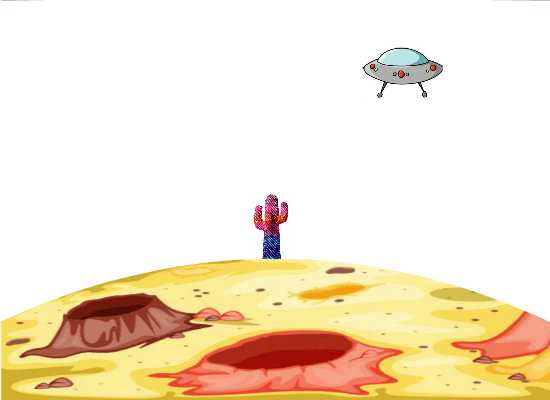
\includegraphics[width=.45\textwidth]{figures/levshina-img3.jpg}
 

\noindent
~\hfill 3.      \hfill     4.\hfill~\\
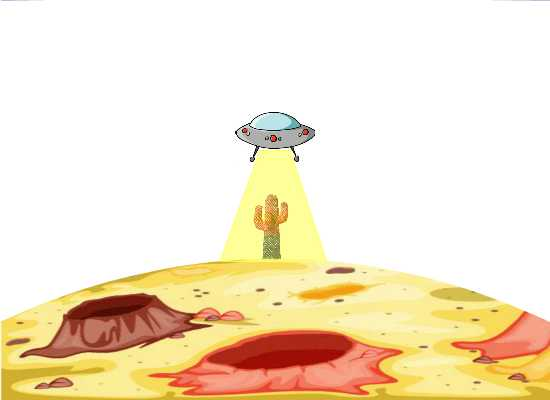
\includegraphics[width=.45\textwidth]{figures/levshina-img4.jpg}

\includegraphics[width=.45\textwidth]{figures/levshina-img5.jpg}
 

\caption{Fragments from one of the video clips.} 
\label{fig:levshina:2}
\end{figure}

\subsection{Participants}

The participants were recruited via my personal network and LinguistList. Most of them had a background in linguistics or languages. After the experiment, they were asked about the aims of the experiment. None of them guessed the true purpose. Overall, I obtained responses from 84 participants. Some of the responses were removed. This was the case if the participants did not follow the training procedure instructions (e.g. a participant did not type in the training sentences), or if the output was unanalysable. As a result, I had 554 valid data points from 70 participants. 

The participants with valid responses had different L1s, but mostly had a Slavic and Germanic linguistic background. There were 40 native Czech speakers, 12 native German speakers, 7 native English speakers, 2 Dutch speakers, 2 Italian speakers, as well as native speakers of Brazilian Portuguese, Croatian, Danish, Polish, Russian, Slovak and Turkish. None of these languages has productive causative prefixes.

\subsection{Results of the artificial language learning experiment}

The counts aggregated across all participants are presented in \tabref{tab:levshina:1}. Lexical and spelling errors were ignored. \figref{fig:levshina:3}, which visualizes these counts, shows that there is a difference between the proportions of short and long forms expressing the frequent and rare causing events. The short forms are overall more preferred than the long ones, but the situations with the more frequent causing event are more frequently expressed by the short forms in comparison with the situations that involve the rare causing event, where the proportions of the short and long forms are almost equal.

\begin{table}
\begin{tabularx}{.8\textwidth}{XSS@{\qquad\qquad}r} 
\lsptoprule
& Frequent & Rare &  {Total}\\
\midrule
Short & 168 & 137 &  {305}\\
Long & 109 & 140 &  {249}\\
\midrule 
 {Total} &  {277} &  {277} &  {554}\\
\lspbottomrule
\end{tabularx} 
\caption{The number of forms selected and their marginal sums.}
\label{tab:levshina:1}
\end{table}

  

\begin{figure}
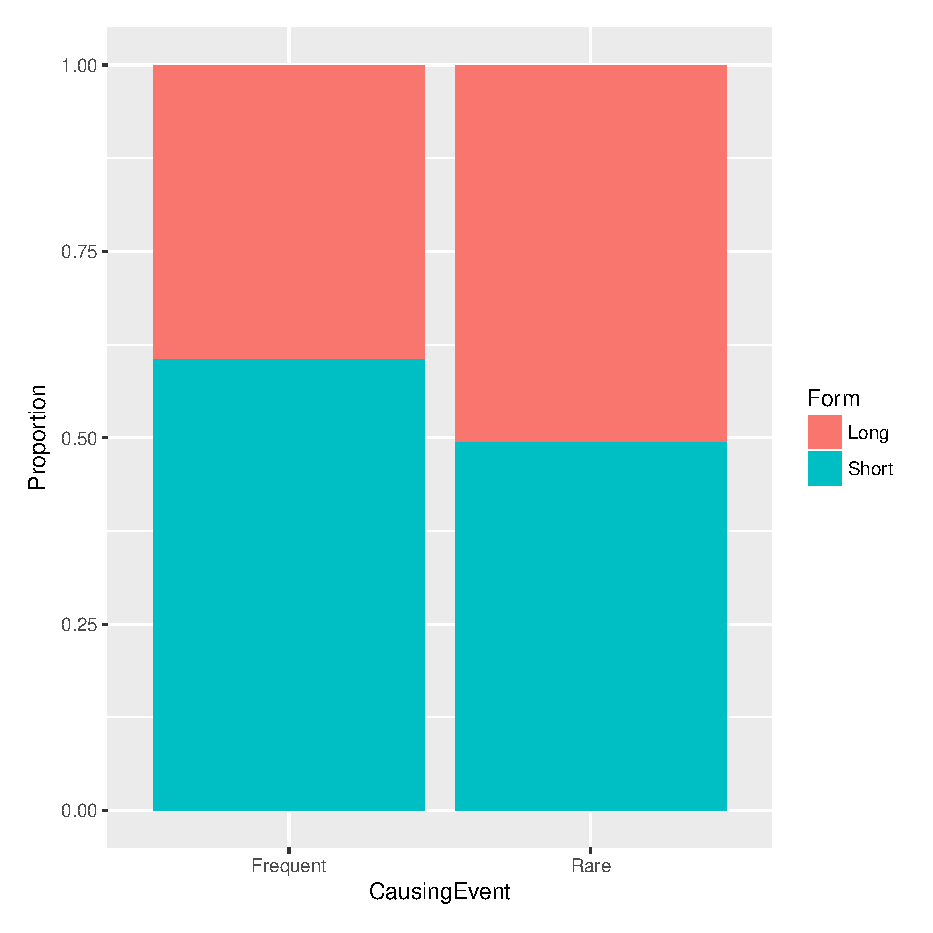
\includegraphics[height=.45\textheight]{figures/Figure3.eps}

% \begin{tikzpicture}
% \begin{axis}[
%     ybar stacked,
% 	bar width=20mm,
% %     enlargelimits=0.15,
% % 	nodes near coords,
%     ymin = 0,
%     ymax = 1, 
%     legend style={at={(1.01,0.70)},
%       anchor=west,legend columns=1},
%     ylabel={Proportion},
%     symbolic x coords={Frequent, Rare},
%     xtick=data,
%     xlabel=Causing Event,
%     reverse legend,
%     x axis line style={draw=none},
% %     ticks = none
%     ]
% \addplot+[ybar,lsLightBlue] plot coordinates {(Frequent,.60) (Rare,.48)};
% \addplot+[ybar,lsLightWine] plot coordinates {(Frequent,.40) (Rare,.52)};
% \legend{Short, Long}
% \end{axis}
% \end{tikzpicture}
\caption{Proportions of short and long forms.}
\label{fig:levshina:3}
\end{figure}

A closer look at the individual subjects’ preferences reveals that most of them use both long and short forms. Seven subjects produced only the short forms. There were no subjects who always preferred the long forms. The distribution is shown in \figref{fig:levshina:4}. 

  

\begin{figure}

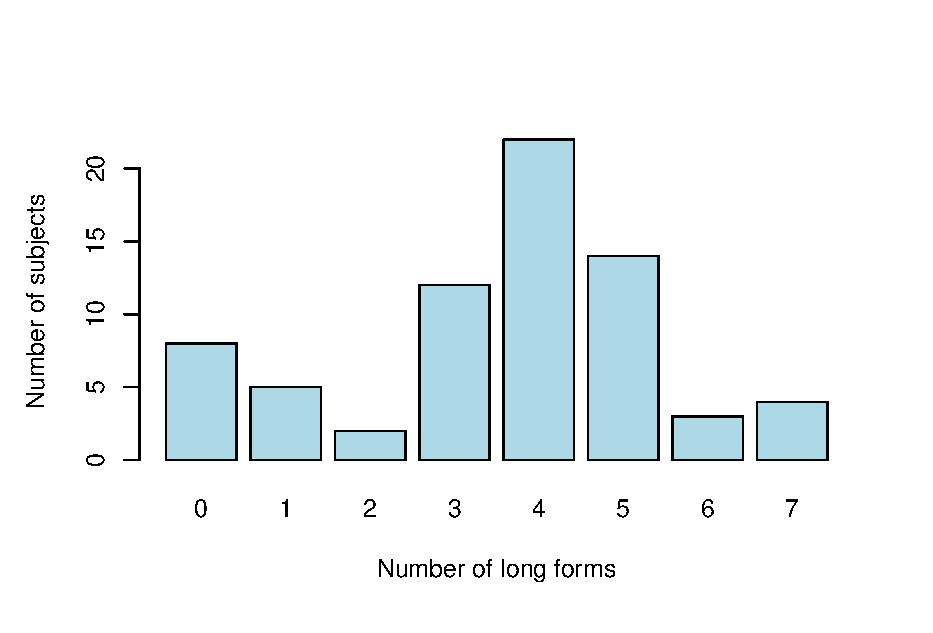
\includegraphics[width=\textwidth]{figures/Figure4.eps}
% 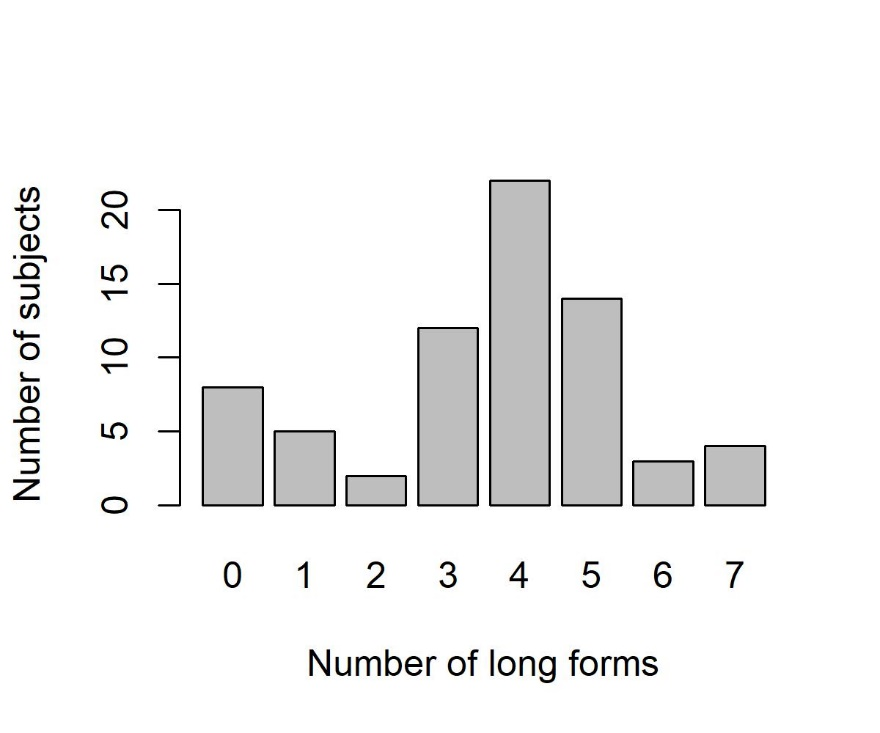
\includegraphics[width=\textwidth]{figures/levshina-img7.jpg} 
%   \langscidata{data/levshina4.csv}
%   \renewcommand{\lspxcol}{j}
%   \begin{tikzpicture}
%     \begin{langscibars}[xlabel=Number of long forms, ylabel=Number of subjects, xtick style={draw=none},ymax=8]
% 	\langscibar{Subjects} 
%     \end{langscibars} 
%   \end{tikzpicture} 
\caption{Individual preferences for the long and short forms}
\label{fig:levshina:4}
\end{figure}

% \begin{figure} 
%   \langscidata{data/dataset1.csv}
%   \begin{tikzpicture}
%     \begin{langscibars}
% 	\langscibar{English}
% 	\langscibar{Spanish}
% 	\langscibar{French}
% 	\langscibar{Italian} 
%     \end{langscibars} 
%   \end{tikzpicture}
%   \caption{Barplot from dataset}
% \end{figure}


The main question, however, is whether the choice of forms is influenced by the type of causing event. In order to test this, I fit a generalized linear mixed-effects model with logit as the link function (R package \textit{lme4}, function \textit{glmer}, \citealt{BatesEtAl2015}). The type of prefix – long or short – was the response variable. The individual participants were treated as random effects (intercepts). There is a significant effect of the type of causing event: if the event is rare, the odds of the longer form to be chosen are 1.66 times greater than when the event is frequent (log-odds ratio \textit{b} = 0.501, \textit{p} = 0.006). This result supports the hypothesis that speakers have a bias towards the use of shorter forms to represent more frequent situations, and longer forms to represent less frequent situations. Random slopes, which represented individual differences in the effect of the predictor on the response, were tested as well, but they did not improve the explanatory power of the model. 

The likelihood ratio test, a standard tool for variable selection and model comparison in regression analysis, demonstrates that the caused event does not have a significant effect on the choice of form (\textit{p} = 0.84), and does not interact with the type of causing event (\textit{p} = 0.6). This means that lexical conditioning can be excluded (cf. \citealt{SmithWonnacott2010}). 

\section{Discussion}\label{sec:levshina:4}

This paper has provided an overview of the applications of the artificial language learning paradigm in testing universal biases suggested by functional and cognitive linguists. One of them, known as the principle of economy, was tested in an online experiment. The results demonstrate that frequent causative situations are more commonly expressed by shorter forms, whereas the subjects are more tolerant of longer forms when expressing rarer causative situations. Therefore, the results of previous corpus-based studies, typological evidence and experimental approaches converge. The fact that the effect was detected in a non-iterative experiment with only one “generation” of language learners, suggests that the bias is very strong.

An important question remains about the nature of this bias and its place in \citegenv{Haspelmath2019tv} classification. Can it be characterized as a functional-adaptive, acquisitional, mutational or maybe even representational constraint? The mutational type can be discarded because we do not have any qualitative changes in the constructions (e.g. possessed nouns becoming adpositions). As for representational constraints, they reflect the properties of the innate language faculty. Even if we accept that economy is an innate principle, since humans and other species are genetically programmed to gain maximal benefits from their behaviour at minimum costs (cf. \citealt{ParkerSmith1990}), it represents a domain-general bias that is not restricted to human language only. There is evidence that the evolution of sense organs and brains is driven by the need to minimize the energy spent for each bit of information received from the environment \citep[3]{Stone2015}. This is why linguistic economy is not a part of Universal Grammar in the generativist sense. 

Thus, we are left with the functional-adaptive and acquisitional types. Although \citetv{Haspelmath2019tv} defines the latter as related to L1 by children only, the overview presented in \sectref{sec:levshina:2} demonstrates that learnability constraints can also be detected in artificial language learning by children and adults. \sectref{sec:levshina:2} also showed that a clear distinction between communicative efficiency and learnability is often problematic within the artificial language learning paradigm. Similar to \citegen{Slobin1996} famous “thinking for speaking”, we can also speak about “learning for using”. This makes the task of distinguishing between these types very difficult. My preliminary answer is that we are dealing with a functional-adaptive constraint because it helps to optimize communication, even though there is no immediate interaction in the experiment. Obviously, more research with a clearer separation between the learning and communication stages is needed. The most pertinent question at this stage is the following: Is it easier to learn a more communicatively efficient language, in which frequent meanings are expressed by shorter forms, and rare functions are expressed by longer forms, than a less efficient one, in which frequent meanings are expressed by longer forms and rare ones by shorter forms?

The artificial language learning paradigm, as I tried to demonstrate in this paper, represents a valuable addition to the toolkit of typologists and functional linguists. However, there are a few caveats that need to be mentioned. First, the experiments involve very limited interaction, if any, in an artificial context. Second, the populations are extremely small. Third, even when a fully artificial language is used, one cannot exclude transfer effects from real language. For example, \citet{Goldberg2013}, in her critical evaluation of Culbertson et al.’s (2012) study of Greenberg’s Universal 18, argues that the word orders Adj + N and N + Adj can be transferred either from English (e.g. \textit{a} \textit{blue} \textit{bird} vs. \textit{something} \textit{red}, \textit{all} \textit{things} \textit{nice}) or from the Spanish-type languages. Note, however, that Culbertson et al. studied a specific formal pattern. As we move to more abstract properties of language or communicative behaviour, such as compositionality or economy, it becomes more difficult to explain these properties by transfer from real languages, although one cannot exclude a possibility that these biases represent very abstract generalizations from the users’ experience with language, and their intuitive expectations about what a “normal” human language should be like. This uncertainty will probably always loom until we find a real alien and have it learn an artificial language. 

\section*{Acknowledgements}

This project has received funding from the European Research Council (ERC) under the European Union's Horizon 2020 research and innovation programme (grant agreement n° 670985). I’m extremely grateful to all colleagues who patiently participated in the experiment, helped to improve the design and to recruit the participants, especially to my good friends from Olomouc university, Michaela Martinkova and Marketa Janebova. All usual disclaimers apply.

\sloppy
\printbibliography[heading=subbibliography,notkeyword=this] 
\end{document}